% presentation
\documentclass{beamer}

\usetheme{Warsaw}

% rus lang
\usepackage[main=russian,english]{babel}

% insert images
\usepackage{wrapfig}
\usepackage{graphicx}
\graphicspath{{./img/}}

% declare operator
\DeclareMathOperator*{\argmin}{argmin} % thin space, limits underneath in displays
\newcommand{\at}[2][]{#1|_{#2}}

% math
\newtheorem{rustheorem}{Теорема}
\usepackage{amsmath}
\DeclareMathOperator{\sign}{sign}
\DeclareMathOperator{\K}{K}
\DeclareMathOperator{\R}{\mathbb{R}}
\DeclareMathOperator{\X}{\mathbb{X}}
\DeclareMathOperator{\Y}{\mathbb{Y}}

\title[Деревья решений]{Лекция 6. Деревья решений}
\subtitle{Основы интеллектуального анализа данных}
\author{Полузёров Т. Д.}
\institute{БГУ ФПМИ}
\date{}

\begin{document}
	
	\begin{frame}
		\titlepage
	\end{frame}
	
	
	\begin{center}
		\frametitle{Структура лекции}
		% \tableofcontents	
	\end{center}
    
	\begin{frame}
		\frametitle{Пример дерева решений}
		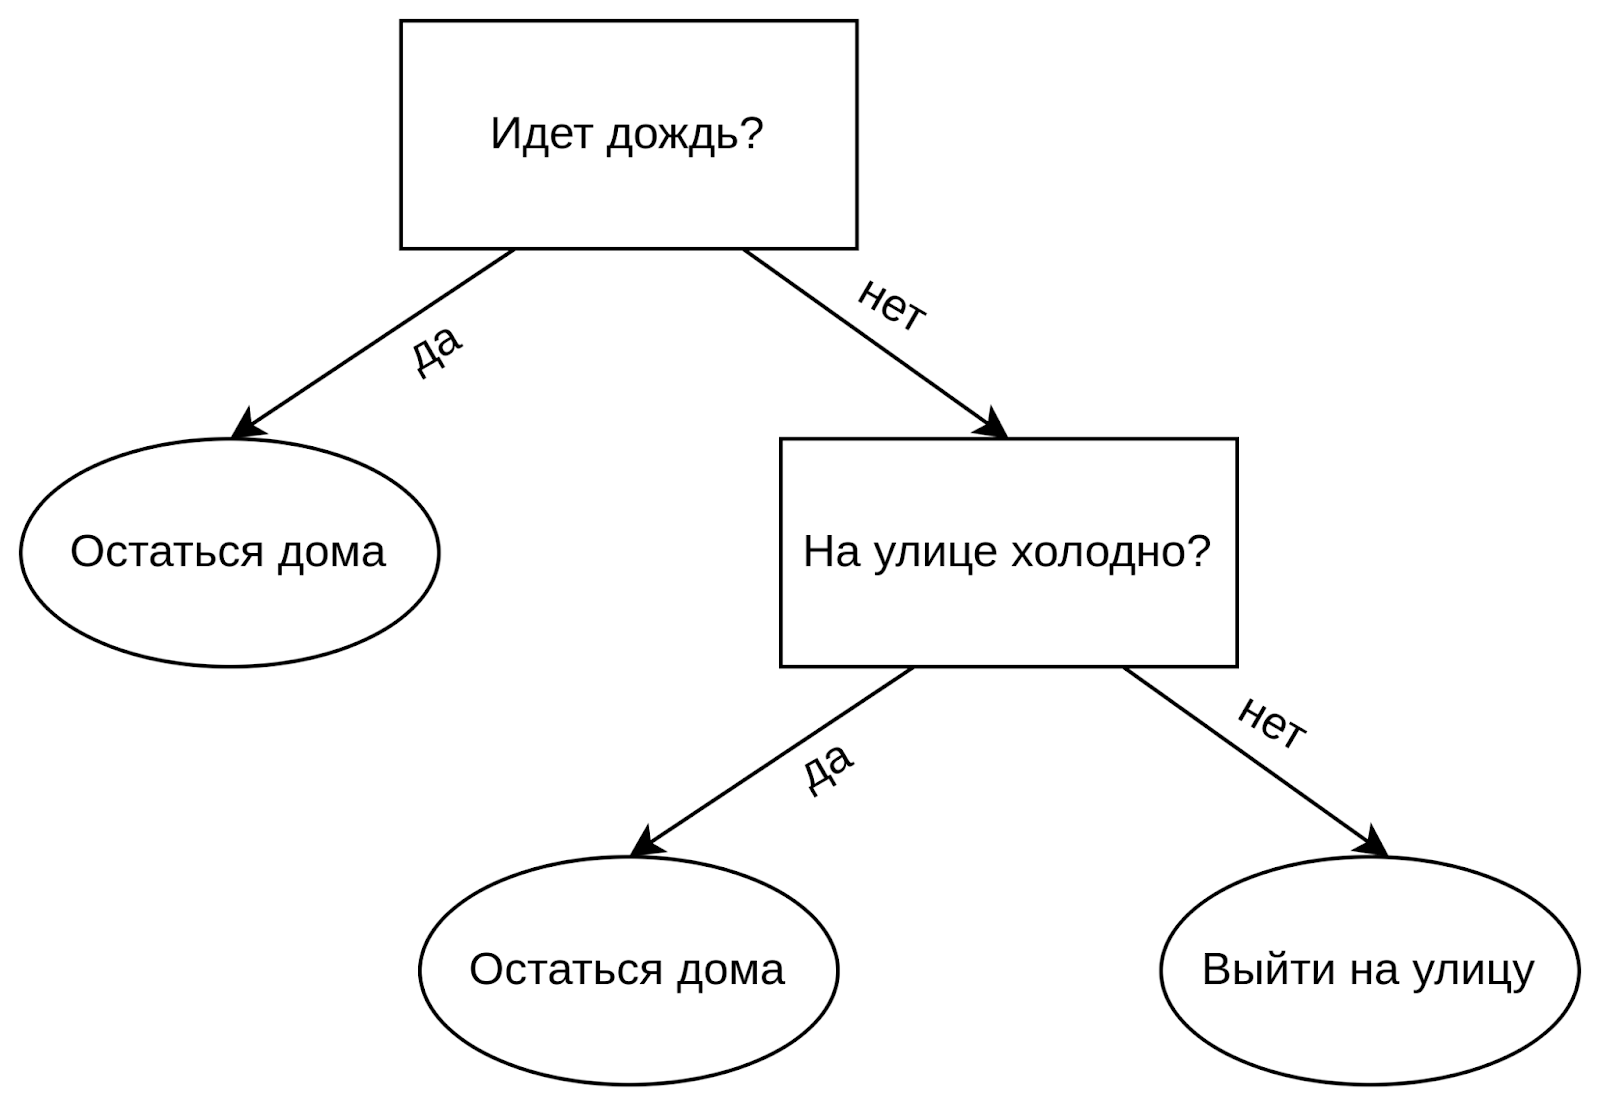
\includegraphics[width=1\textwidth]{dc}
	\end{frame}

    \begin{frame}
        \frametitle{Компоненты бинарного дерева}

		Дерево $T$ состоит из 2-х типов вершин:
		\begin{itemize}
			\item \textbf{Внутрення} вершина $v$ хранит в себе предикат $b_v: \X \rightarrow \{0, 1\}$
			\item \textbf{Листовая вершина} $v$ хранит выходное значение $c_v \in \Y$
		\end{itemize}

		\vspace{15pt}

		Алгоритм $a(x)$ работает по схеме:
		\begin{enumerate}
			\item Стартуем из корня
			\item Вычисляем предикат в текущей вершине
			\item Если $b_v = 1$ - шагаем в право, $b_v = 0$ - в лево
			\item Пока не дошли до листовой вершини, повторяем с шага 2
			\item Возвращаем значение в листе $c_v$
		\end{enumerate}
    \end{frame}

	\begin{frame}
		\frametitle{Предикаты}

		Предикат - любая решащая функция $b :\X \rightarrow \{0, 1\}$
		
		\vspace{15pt}

		\begin{itemize}
			\item Пороговая функция $b(x) = [x_i > t]$
			\item Линейный $b(x) = [\langle x, \omega \rangle > t]$
			\item Метрический $b(x) = [\rho(x, x_v) > t]$, где $x_v$ - некоторый объект выборки
		\end{itemize}

		\vspace{15pt}

		Но выбор сложных предикатов - излишен. Поэтому используются $b(x) = [x_i > t]$
	\end{frame}

	\begin{frame}
		\frametitle{}
		

	\end{frame}

\end{document}
